\chapter{代数拓扑}
% \section{同调论}
%     \subsection{Brouwer不动点定理与Sperner引理}
%     我们首先叙述 Brouwer不动点定理与Sperner引理:
%     \begin{theorem}[Brouwer不动点定理]
%         设 $f$ 是 $n$ 维闭球 $B^n$ 到自身的连续映射, 则 $f$ 必有不动点.
%     \end{theorem}
%     \begin{lemma}[Sperner引理]
%         设 $K=[v_0,\dots,v_n]$ 是 $n$ 维单纯形, 
%         考虑其三角剖分 $T$, 将 $T$ 的顶点 $(n+1)$ 染色, 
%         即定义 $\lambda:V(T)\rightarrow\{0,\dots,n\}$, 且满足对任意指标子集
%         $\{i_0,\dots,i_k\}\subseteq\{0,\dots,n\}$, 
%         $\lambda$ 在 $[v_{i_0},\dots,v_{i_k}]$ 上的限制的值域包含于 
%         $\{i_0,\dots,i_k\}$. 则一定存在 $u_0,\dots,u_n\in V(T)$, 
%         使得 $[u_0,\dots,u_n]$ 是三角剖分 $T$ 的单形, 
%         且 $\lambda(u_i)$ 互不相同.
%         \begin{figure}[hbtp]
%             \centering
%             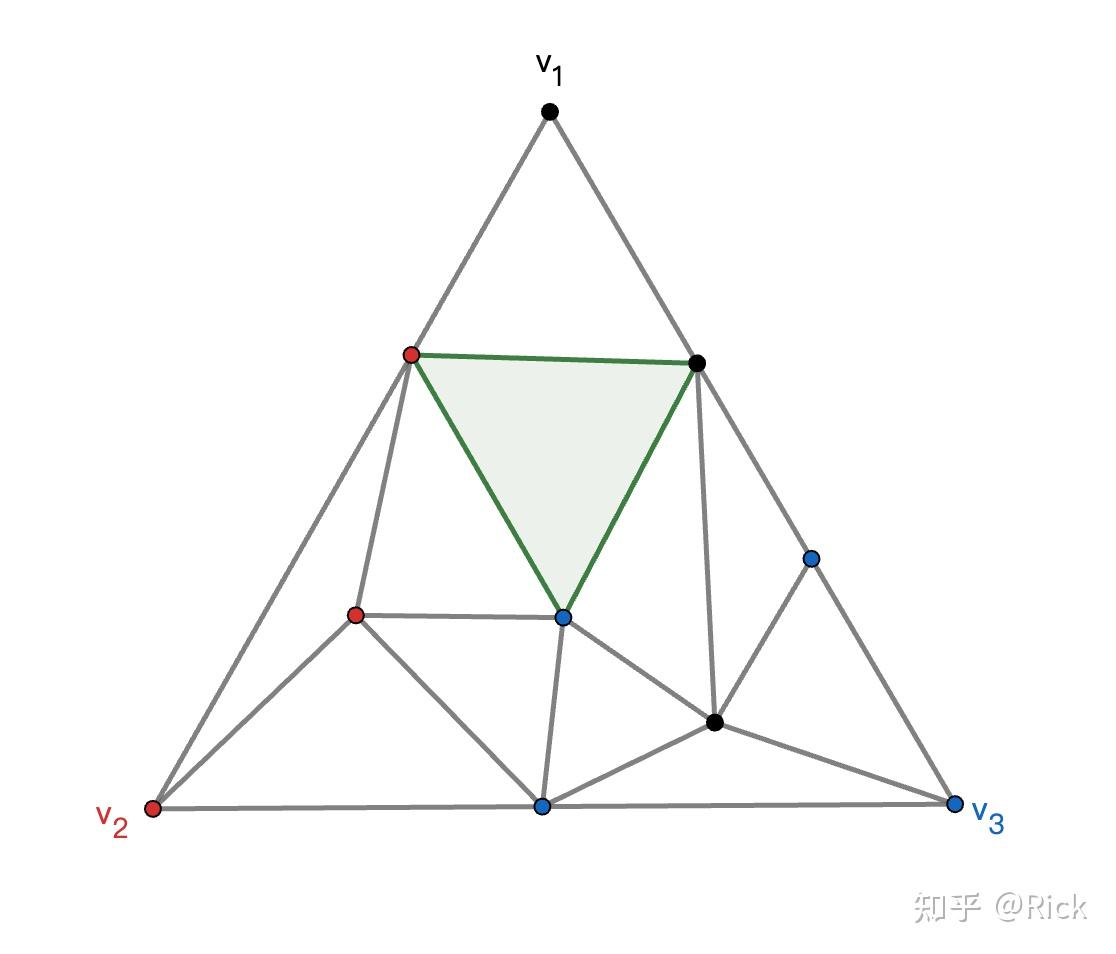
\includegraphics[scale=0.2]{Figures/SpernerLemma.jpg}
%             \caption[SpernerLemma]{Sperner引理示意图}
%         \end{figure}
%     \end{lemma}

%     它们一个是拓扑的定理, 一个是组合的定理, 看似没有联系, 
%     但实际上我们能证明它们是等价的: 
%     \begin{proof}[{\bf 等价性的证明}]
%         由于 $B^n\cong K$, 我们将 Brouwer不动点定理的叙述改为 
%         $K$ 到自身的连续映射 $f$ 必有不动点.

%         $1^{\circ}$:Sperner引理 $\Rightarrow$ Brouwer不动点定理
        
%         设 $K = [v_0,\dots,v_n]$ 是 $n$ 维单形, 对 $\forall x\in K$, 
%         $x=\sum_i\alpha_iv_i,\,\alpha_i\geqslant0,\,\sum_i\alpha_i=1$. 
%         设 $f(x) = \sum_i\beta_iv_i$, 定义染色映射 
%         $\lambda(x)$ 为使得 $\alpha_i\geqslant\beta_i$ 
%         且 $\alpha_i\neq0$ 的最小下标 $i$. 
%         我们首先观察到在任意集合 $\{i_0,\dots,i_k\}\subseteq\{0,\dots,n\}$ 中, 
%         对 $\forall x\in[v_{i_0},\dots,v_{i_k}]$, $x$ 的坐标 $\alpha$ 满足 
%         $\alpha_i=0,\,i\notin\{i_0,\dots,i_k\}$, 
%         因此 $\lambda(x)$ 只可能在 $\{i_0,\dots,i_k\}$ 中取值.

%         固定染色 $\lambda$, 取重心重分 $K^0,K^1,\dots$, 
%         则在每一个 $K^j$ 中 $\lambda$ 均满足引理条件, 
%         于是存在异色单形 $\Delta^j=[u^j_0,\dots,u^j_n]$, 
%         不妨设 $\lambda(u^j_i)=i$.
%         因为 $K$ 是紧集, 因此 $\{u^j_0\}_j$ 存在收敛子列, 
%         不妨设就为序列本身, 由重心重分的性质知 $\Delta^j$ 的直径趋于零, 
%         因此对所有 $i$, $\{u^j_i\}_j$ 均收敛于同一点 $u$, 即 
%         $u=\lim\limits_{j\rightarrow\infty}u^j_i,\,\forall\,i=0,\dots,n$. 
%         由染色的定义知 $u^j_i$ 的 $v_i$ 坐标不等于零且大于等于 $f(u^j_i)$ 的, 
%         根据极限的保号性知 
%         $u$ 的所有坐标 $\alpha_i$ 大于等于 $f(u)$ 对应的坐标 $\beta_i$, 
%         但因为 $\sum_i\alpha_i = \sum_i\beta_i = 1$, 
%         所以 $\alpha_i=\beta_i$, 因此 $u = f(u)$ 是 $f$ 的不动点.

%         $2^{\circ}$:Sperner引理 $\Leftarrow$ Brouwer不动点定理
        
%         设 $K = [v_0,\dots,v_n]$ 是 $n$ 维单形, 
%         $\lambda$ 为满足引理要求的染色, $T$ 是 $K$ 的一个三角剖分, 
%         则可以定义单纯映射 $f:K\rightarrow K$ 如下: 对 $\forall x\in V(T)$, 
%         定义 $f(x) = v_{\lambda(x)}$, 若 $x = \sum_{i=0}^{k}\alpha_ix_i$, 
%         其中 $[x_0,\dots,x_k]$ 为 $T$ 的 $k$ 维单形, 
%         定义 $f(x) = \sum_{i=0}^{k}\alpha_iv_{\lambda(x_i)}$.

%         若 $T$ 中没有 $n$ 维异色单形, 则 $f$ 的像集包含于 $\partial K$ 中, 
%         且对于每个 $(n-1)$ 维面 $[v_0,\dots,\hat{v_i},\dots,v_n]$ 均有 
%         $f([v_0,\dots,\hat{v_i},\dots,v_n])\subset[v_0,\dots,\hat{v_i},\dots,v_n]$.
%         不妨设 $\sum_{i=0}^{n}v_i = 0$, 即 $K$ 的重心是原点. 
%         定义 $g:\partial K\rightarrow \partial K$, 
%         $g(x)$ 为射线 $xO$ 与 $\partial K$ 的另一个交点, 类比对径映射. 
%         则 $g([v_0,\dots,\hat{v_i},\dots,v_n])\cap[v_0,\dots,\hat{v_i},\dots,v_n]=\emptyset$
%         则 $g\circ f$ 是 $K$ 到自身的连续映射, 但没有不动点, 
%         与Brouwer不动点定理矛盾.
%     \end{proof}
    
%     现在我们回到Sperner引理本身的证明
%     \begin{proof}
%         对维数 $n$ 做归纳, 我们证明对任意维数异色单形的个数均为奇数.

%         当 $n=1$ 时, $K = [v_0,v_1]$ 可看做闭区间 $[0,1]$, 
%         设 $v_0=x_0<x_1<\cdots<x_m=v_1$ 是剖分 $T$ 中的点, 
%         则 $\#\verb|异色单形| = \#\left\{i\,\big|\,\lambda(x_{i-1})\neq\lambda(x_i)\right\}$. 
%         而
%         \begin{equation*}
%             1 = \lambda(v_1)-\lambda(v_0) 
%             = \sum_{i=1}^{m}\lambda(x_i)-\lambda(x_{i-1}) 
%             = \sum_{\lambda(x_{i-1})\neq\lambda(x_i)}\lambda(x_i)-\lambda(x_{i-1})
%         \end{equation*} 
%         因此 $\#\verb|异色单形|$ 是奇数. 

%         假设维数为 $n-1$ 时命题成立, 
%         我们称 $T$ 中的 $(n-1)$ 维单形 $[x_0,\dots,x_{n-1}]$ 为一个好单形, 
%         若 $\{\lambda(x_0),\dots,\lambda(x_{n-1})\} = \{0,\dots,n-1\}$. 
%         对 $T$ 中的  $n$ 维单形
%         $\Delta_n=[u_0,\dots,u_n]$, 令 $c(\Delta_n)$ 为 $\Delta_n$ 中好单形的个数, 
%         记 $S=\{\lambda(u_0),\dots,\lambda(u_n)\}$, 则
%         \begin{equation*}
%             c(\Delta_n)= \left\{
%             \begin{aligned}
%                 0,\; &\{0,\dots,n-1\}\nsubseteq S \\
%                 2,\; &\{0,\dots,n-1\} = S \\
%                 1,\; &\{0,\dots,n\} = S  
%             \end{aligned}\right. ,
%         \end{equation*}
%         于是异色单形个数的奇偶性与 
%         $\sum\limits_{\Delta_n\subset T}c(\Delta_n)$ 的奇偶性相同. 
%         而当好单形在 $\overset{\circ}{K}$ 内时, 它是两个 $n$ 单形的公共面; 
%         当好单形在 $\partial K$ 上时, 它仅为一个 $n$ 单形的面.
%         因此异色单形个数的奇偶性与 $\partial K$ 上好单形的个数的奇偶性相同, 
%         根据条件好单形仅在 $[v_0,\dots,v_{n-1}]$ 中出现, 
%         由归纳假设知 $[v_0,\dots,v_{n-1}]$ 中好单形有奇数个, 命题成立.
%     \end{proof}

%     \subsection[Invariance of domain]{区域不变性定理(Invariance of domain)}
%         该定理也是拓扑中的重要定理, 有人说它是欧式空间的内蕴性质, 
%         用它可以区分不同维数的欧式空间.
%         \begin{theorem}
%             设 $U$ 为 $\mathbb{R}^n$ 中的开子集, 
%             $f:U\rightarrow\mathbb{R}^n$ 为连续单射, 
%             则 $f(U)$ 为 $\mathbb{R}^n$ 的开子集且 $f$ 为开映射, 
%             即 $f$ 为 $U$ 到 $f(U)$ 的同胚.
%         \end{theorem}

%     \subsection[Poincar\'e Lemma]{Poincar\'e Lemma 的另一种表述形式}
%         \begin{lemma}[d-Poincar\'e lemma]
%             若整体有 $\md\omega = 0$, 
%             则方程 $\md\eta=\omega$ 局部有解, 
%             即在每点处存在邻域使得方程有解.
%         \end{lemma}
%         \begin{lemma}[$\overline{\partial}$-Poincar\'e lemma]
%             若整体有 $\overline{\partial}\omega = 0$, 
%             则方程 $\overline{\partial}\eta=\omega$ 局部有解, 
%             即在每点处存在邻域使得方程有解.
%         \end{lemma}
%         \begin{remark}
%             因此若整体有 $\md\omega = 0$, 
%             但方程 $\md\eta=\omega$ 在整体上没有解, 
%             这就表明空间本身限制的整体解的存在性, 
%             也就是说我们检测到一个拓扑上的障碍.
%         \end{remark}

%     \subsection[Excision Theorem in Signular Homology]{切除定理(Excision Theorem)}
%         \begin{theorem}[切除定理表述1]\label{thm:excision-1}
%             设 $Z\subset A\subset X$ 满足 $\overline{Z}\subset A^{\circ}$, 
%             则空间偶的嵌入 $(X-Z,A-Z)\hookrightarrow(X,A)$ 
%             诱导了相对同调群之间的同构:
%             \begin{equation*}
%                 H_n(X-Z,A-Z)\overset{\cong}{\longrightarrow} H_n(X,A),\quad n\geq0.
%             \end{equation*}
%         \end{theorem}
%         这个定理有一个等价的表述:
%         \begin{theorem}[切除定理表述2]\label{thm:excision-2}
%             设 $A,B\subset X$ 且满足 $A^{\circ}\cup B^{\circ}=X$, 
%             则空间偶的嵌入 $(B,A\cap B)\hookrightarrow(X,A)$ 
%             诱导了相对同调群之间的同构:
%             \begin{equation*}
%                 H_n(B,A\cap B)\overset{\cong}{\longrightarrow} 
%                 H_n(X,A),\quad n\geq0.
%             \end{equation*}
%         \end{theorem}
%         \begin{remark}
%             两种表述靠 $B=X-Z\;(Z=X-B)$ 相互转化.
%         \end{remark}

%         为了证明这个定理, 
%         我们需要先证明同调的“局部性”({\bf locality principal}).

%         设 $X$ 是一个拓扑空间, 
%         我们称 $X$ 的子集族 $\mathfrak{U}=\{U_j\}_{j\in J}$ 是一个覆盖, 
%         若 $\{U_j^{\circ}\}_{j\in J}$ 构成一个开覆盖
%         (注意 $U_j$ 本身不必是开集).

%         \begin{definition}[{\bf$\mathfrak{U}$-small chains}]\hfill
%             \begin{itemize}
%                 \item 一个 $n$-单形 $\sigma:\Delta^n\rightarrow X$ 
%                 被称为 $\mathfrak{U}$-small 的, 
%                 若 ${\rm Im}\,\sigma$ 在某个 $U_j$ 中.
%                 \item 一个 $n$-复形 $c=\sum_i{n_i\sigma_i}$ 
%                 被称为 $\mathfrak{U}$-small 的, 
%                 若每个 $\sigma_i$ 都是 $\mathfrak{U}$-small 的.
%                 \item 所有 $\mathfrak{U}$-small 的 $n$-复形构成 
%                 $C_n(X)$ 的一个子群, 记为
%                 \begin{equation*}
%                     C^{\mathfrak{U}}_n(X):=
%                     \left\{c\in C_n(X)\,\big|\,
%                     c \text{ is $\mathfrak{U}$-small}\right\}.
%                 \end{equation*}
%                 \item 若 $A\subset X$, 记
%                 \begin{equation*}
%                     C^{\mathfrak{U}}_n(X,A)
%                     :=\frac{C^{\mathfrak{U}}_n(X)}{C^{\mathfrak{U}}_n(A)}.
%                 \end{equation*}
%             \end{itemize}
%         \end{definition}

%         若记 $\iota_j:U_j\hookrightarrow X$ 为 $U_j$ 到 $X$ 的嵌入, 那么 $C^{\mathfrak{U}}_n(X)$ 也可以被定义为
%         \begin{equation*}
%             C^{\mathfrak{U}}_n(X) = {\rm Im}\left(\bigoplus_{j\in J}C_n(U_j)\xrightarrow{\oplus_j (\iota_{j})_*}C_n(X)\right).
%         \end{equation*}

%         这一概念的关键在于我们可以仅用 $\mathfrak{U}$-small 的链来计算原空间的同调群, 这体现了同调群的局部性.

%         \begin{theorem}[{\bf Locality Principle/Small Chain Theorem}]\label{thm:small-chain}
%             设 $\mathfrak{U}$ 是 $X$ 的一个覆盖, 则链复形的嵌入映射
%             \begin{equation*}
%                 C^{\mathfrak{U}}_n(X)\subset C_n(X)
%             \end{equation*}
%             诱导了同调群之间的同构.
%         \end{theorem}

%         这个定理的证明需要用到重心剖分, 其证明过程有些繁琐, 所以我们跳过该定理的证明, 先看如何用这个定理推导出切除定理.

%         \begin{proof}[{\bf Proof of the Excision Axiom using small chains:}]\hfill
            
%             我们证明切除定理的表述 $2$, 令 $\mathfrak{U} = \{A,B\}$. 链复形的嵌入映射 $C^{\mathfrak{U}}_n(X)\subset C_n(X)$ 诱导了链复形短正合列之间的一个态射:
            
%             \vspace{8pt}
%             \begin{tikzcd}
%                 0 \arrow[r] & C_*(A) \arrow[r] \arrow[d, equal] & C^{\mathfrak{U}}_{*}(X) \arrow[r] \arrow[d] & C^{\mathfrak{U}}_{*}(X)/C_*(A) \arrow[d, dashed] \arrow[r] & 0 \\
%                 0 \arrow[r] & C_*(A) \arrow[r]                                & C_*(X) \arrow[r]                            & C_*(X)/C_*(A) \arrow[r]                                    & 0
%             \end{tikzcd}.
%             \vspace{8pt}

%             因为中间竖直的映射诱导了同调群之间的同构映射(定理\ref{thm:small-chain}), 由根据短正合引长正合、同调群的自然性、五引理, 
%             我们得到右侧竖直映射诱导了同调群的同构, 由此转化为比较 $C_*(B,A\cap B)$ 和 $C^{\mathfrak{U}}_{*}(X)/C_*(A)$.

%             注意到
%             \begin{gather*}
%                 C^{\mathfrak{U}}_{*}(X) = C_*(A)+C_*(B)\subset C_*(X), \\
%                 C_*(A\cap B) = C_*(A)\cap C_*(B).
%             \end{gather*}
%             因此
%             \begin{equation*}
%                 \frac{C_*(B)}{C_*(A\cap B)}=\frac{C_*(B)}{C_*(A)\cap C_*(B)}\cong\frac{C_*(A)+C_*(B)}{C_*(A)}=\frac{C^{\mathfrak{U}}_{*}(X)}{C_*(A)}.
%             \end{equation*}
%             中间的同构源自同态基本定理. 

%             因此链映射
%             \begin{equation*}
%                 C_*(B,A\cap B)\rightarrow C_*^{\mathfrak{U}}(X)/C_*(A)
%             \end{equation*}
%             诱导了同调群之间的同构, 原命题成立.
%         \end{proof}

%         \begin{proof}[{\bf Proof of Locality Principle}]\footnote{证明源自 Hacter 的 Algebraic Topology, 此处是我总结凝练的个人理解.}
%             我们需要引入重心重分(或叫重心剖分)这一操作, 需要分几步定义:

%             \noindent {\bf Step 1:} 首先定义什么是 $n$-单形 $\Delta^n$ 的重心重分. 为了方便我们使用坐标描述, 
%             我们将 $\Delta^n$ 嵌入底空间 $\mathbb{R}^n$, 可用顶点集表示为 $[\ft{v}{0}{n}]$, 
%             其中的点可以表示为 $P = \sum_{i=0}^{n}t_iv_i$, $0\leq t_i\leq 1,\;\sum_{t_0}^{n}t_i=1$ 是点 $P$ 的 $n+1$ 个坐标.
            
%             我们知道从几何图形上看 $\Delta^n$ 重心重分后是一些更小块的 $n$-单形(带符号),
%             但是为了规范叙述重心重分, 我们需要将重分后的对象视为 $LC_n(Y)$ 中的元素, 其中 $Y$ 是某个欧氏空间中的凸集\footnote{这里我很纠结到底用不用书上的记号, 我原本想把每个 $\Delta^n$ 视为 $C_n(\Delta^n)$ 中的元素, 但这样得不到一个链复形, $S$ 和 $T$ 无法定义在一个统一的 $C_*(?)$. 加上线性映射这一条件也是必要的, 否则映射的像就不是规则的图形了.}. 
%             也即, 我们把原始的 $\Delta^n$ 视为 $\id:\Delta^n\rightarrow\Delta^n$, 重分后得到 $S\Delta^n\in LC_n(Y)$.

%             \noindent$\mathbf{1}^{\circ}$ 锥映射(cone map): 设 $b$ 是 $\mathbb{R}^{n}$ 中的某一个点, 定义以 $b$ 为顶点的锥映射, 写为
%             \begin{equation*}
%                 b:[\ft{v}{0}{n}]\mapsto[b,\ft{v}{0}{n}]
%             \end{equation*}
%             因此 $b([\ft{v}{0}{n}])$ 中坐标为 $(\ft{t}{0}{n+1})$ 的点是 
%             \begin{equation*}
%                 t_0b+\sum_{t=1}^{n+1}t_iv_i=t_0b+\left(1-t_0\right)\sum_{t=1}^{n+1}\dfrac{t_i}{1-t_0}v_i. 
%             \end{equation*}

%             \noindent$\mathbf{2}^{\circ}$ 重心重分映射 $S:LC_n(\Delta^n)\rightarrow LC_n(\Delta^n)$. 
%             设 $\lambda$ 是一个 $n$-单形, 记 $b_\lambda$ 为 $\lambda$ 的重心, 即所有坐标都取 $\frac{1}{n+1}$ 的点. 我们归纳地定义
%             \begin{equation*}
%                 S\lambda=
%                 \begin{cases}
%                     [\varnothing] &, n = -1;\\
%                     b_{\lambda}S(\partial\lambda) &, n \geq 0.
%                 \end{cases}
%             \end{equation*}
%             $S$ 在小维数单形上的作用:
%             \begin{itemize}
%                 \item 当 $n=-1$, 即 $\lambda=[\varnothing]$ 时, $S[\varnothing] = [\varnothing]$; 
%                 \item 当 $n=0$, 即 $\lambda=[w_0]$ 时, $b_\lambda=w_0$, $S[w_0] = w_0S\partial[w_0] = w_0([\varnothing]) = [w_0]$;
%                 \item  当 $n=1$, 即 $\lambda=[w_0,w_1]$ 时, $S[w_0,w_1] = b_{\lambda}S([w_1]-[w_0]) = [b_{\lambda},w_1]-[b_{\lambda},w_0]$.
%             \end{itemize}
%             下面归纳地证明 $S$ 是链映射, 即 $S\partial=\partial S$.
%             \begin{itemize}
%                 \item 当 $n=-1,0$ 时, $S = \mathbbm{1}$, 等式显然成立.
%                 \item 当 $n>0$ 时, 
%                 \begin{align*}
%                     \partial S\lambda &= \partial b_\lambda(S\partial\lambda) \\
%                     &= S\partial\lambda-b_\lambda\partial(S\partial\lambda) \qquad \text{因为}\; \partial b_\lambda=\mathbbm{1}-b_\lambda\partial \\
%                     &= S\partial\lambda-b_\lambda(S\partial\partial\lambda) \qquad \text{因为归纳假设}\; \partial S(\partial\lambda) = S\partial(\partial\lambda) \\
%                     &= S\partial\lambda \qquad \text{因为}\; \partial\partial=0.
%                 \end{align*}
%             \end{itemize}

%             \noindent$\mathbf{3}^{\circ}$ $\id$ 和 $S$ 的链同伦 $T:C_n(Y)\rightarrow C_{n+1}(Y)$, 我们归纳地定义
%             \begin{equation*}
%                 T\lambda = 
%                 \begin{cases}
%                     0 &, n = -1; \\
%                     b_{\lambda}(\lambda-T\partial\lambda) &, n\geq0.
%                 \end{cases}
%             \end{equation*}
%             \begin{center}
%                 \begin{tikzcd}[column sep=1.8em]
%                     \cdots \arrow[r] & LC_{2}(Y) \arrow[r] \arrow[d, "S"] & LC_{1}(Y) \arrow[r] \arrow[d, "S"] \arrow[ld, "T"'] & LC_{0}(Y) \arrow[r] \arrow[d, "S"', "\mathbbm{1}"] \arrow[ld, "T"'] & LC_{-1}(Y) \arrow[r] \arrow[d, "S"', "\mathbbm{1}"] \arrow[ld, "T"', "0"] & 0 \\
%                     \cdots \arrow[r] & LC_{2}(Y) \arrow[r]                & LC_{1}(Y) \arrow[r]                                 & LC_{0}(Y) \arrow[r]                                         & LC_{-1}(Y) \arrow[r]                                              & 0
%                 \end{tikzcd}
%             \end{center}
%             $T$ 在小维数单形上的作用:
%             \begin{itemize}
%                 \item  当 $n=-1$, 即 $\lambda=[\varnothing]$ 时, $T[\varnothing] = 0$; 
%                 \item 当 $n=0$, 即 $\lambda=[w_0]$ 时, $b_\lambda=w_0$, $T[w_0] = w_0([w_0]-T\partial[w_0]) = w_0([w_0]) = [w_0.w_0]$;
%                 \item  当 $n=1$, 即 $\lambda=[w_0,w_1]$ 时, $T[w_0,w_1] = b_{\lambda}\Big([w_0,w_1]-T([w_1]-[w_0])\Big) = [b_{\lambda},w_0,w_1]-[w_1,w_1]+[w_0,w_0]$.
%             \end{itemize}
%             $T$ 的几何解释如下: 将 $\Delta^n\times I$ 分成若干个 $\Delta^n$, 满足下底 $\Delta^n\times\{0\}$ 仍为一整个 $\Delta^n$(代表 $\id$), 
%             上底则成为重心重分后的图形(代表 $S\Delta^n$). $T$ 作用在某个 $\lambda$ 上可能会出现 $[w_0,w_0]$ 这样的元素, 
%             对此我们可以将前一个 $w_0$ 视作时间参数 $t=1$ 的点, 后一个视作 $t=0$ 的点, 通过人为增添一个时间维度(即乘以 $I$), 我们能更好地想象 $T$ 的几何动机, 
%             $T$ 实际作用的像是前文描述的图形在投影 $\Delta^n\times I\rightarrow\Delta^n$ 下的像.
%             \begin{figure}[hbtp]
%                 \centering
%                 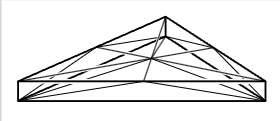
\includegraphics{./Figures/重心重分与恒同的链同论.png}
%                 \caption{重心重分与恒同的链同论}
%                 \label{figure:chain_homo_T}
%             \end{figure}
%             下面归纳地验证 $T$ 是连接 $\id$ 和 $S$ 的链同论, 即 $\partial T+T\partial=\mathbbm{1} - S$:
%             \begin{itemize}
%                 \item 当 $n=-1$ 时, $S = \mathbbm{1}, T=0$, 显然成立.
%                 \item 当 $n\geq0$ 时, 
%                 \begin{align*}
%                     \partial T\lambda &= \partial b_\lambda(\lambda-T\partial\lambda) \\
%                     &= (\lambda-T\partial\lambda) - b_\lambda\partial(\lambda-T\partial\lambda)\qquad\text{因为}\;\partial b_\lambda=\mathbbm{1}-b_\lambda\partial \\
%                     &= \lambda-T\partial\lambda - b_\lambda\partial\lambda + b_\lambda\partial T\partial\lambda \\
%                     &= \lambda-T\partial\lambda - b_\lambda\partial\lambda + b_\lambda(\partial\lambda - S\partial\lambda - T\partial\partial\lambda)\qquad\text{因为归纳假设} \\
%                     &= \lambda-T\partial\lambda - b_\lambda(S\partial\lambda) \\
%                     &= \lambda - S\lambda - T\partial\lambda.
%                 \end{align*}
%             \end{itemize}

%             \noindent {\bf Step 2:} 对一般的链 $\sigma:\Delta^n\rightarrow X$ 定义重心重分.

%             \noindent$\mathbf{1}^\circ$ 定义 $S:C_n(X)\rightarrow C_n(X)$ 为
%             \begin{equation*}
%                 S\sigma=\sigma_\sharp S\Delta^n
%             \end{equation*}
%             下面的示意图能帮助我们理解 $S$ 的定义.(图有问题, 需要修正)
%             % \begin{figure}[hbtp]
%             %     \centering
%             %     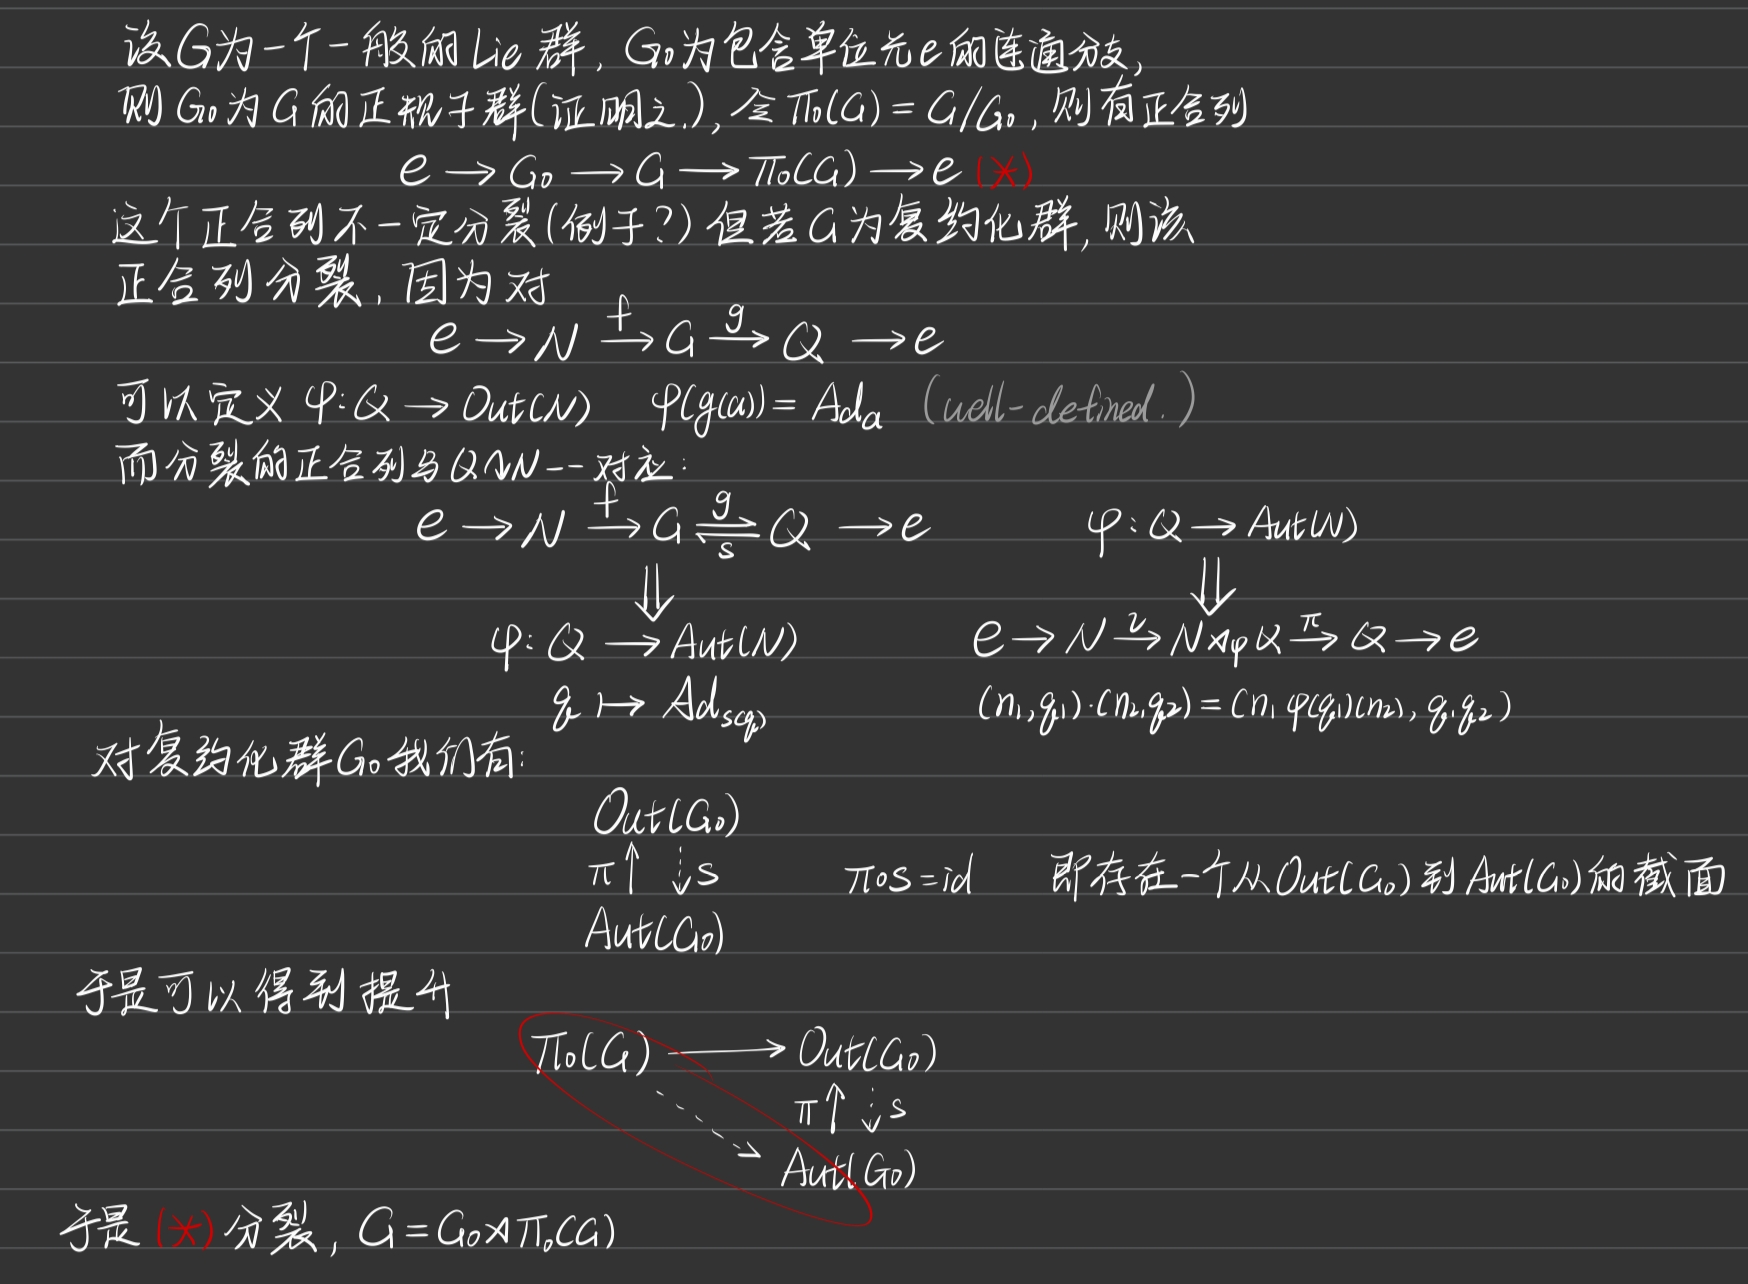
\includegraphics[scale=0.2]{./Figures/20240926-223647.jpg}
%             %     \caption{重心重分与恒同的链同论}
%             %     \label{figure:general_S}
%             % \end{figure}
%             下面验证 $S$ 是一个链映射, 即 $\partial S = S\partial$:
%             \begin{align*}
%                 \partial S\sigma &= \partial\sigma_\sharp S\Delta^n = \sigma_\sharp\partial S\Delta^n = \sigma_\sharp S\partial\Delta^n \\
%                 &= \sigma_\sharp S\sum_{i=0}^{n}(-1)^i\Delta^n_i \\
%                 &= \sum_{i=0}^{n}(-1)^i\sigma_\sharp S\Delta^n_i \\
%                 &= \sum_{i=0}^{n}(-1)^i S(\sigma|_{\Delta^n}) \\
%                 &= S\left(\sum_{i=0}^{n}(-1)^i \sigma|_{\Delta^n}\right) = S(\partial\sigma).
%             \end{align*}
%             \noindent$\mathbf{2}^\circ$ 类似地定义 $T:C_n(X)\rightarrow C_{n+1}(X)$ 为
%             \begin{equation*}
%                 T\sigma=\sigma_\sharp T\Delta^n
%             \end{equation*}
%             下面验证 $T$ 是一个链同伦, 即 $\partial T + T\partial = \mathbbm{1} - S$:
%             \begin{align*}
%                 \partial T\sigma &= \partial\sigma_\sharp T\Delta^n = \sigma_\sharp\partial T\Delta^n \\
%                 &= \sigma_\sharp(\mathbbm{1}-S - T\partial)\Delta^n \\
%                 &= \sigma-S\sigma-\sigma_\sharp T\partial\Delta^n\qquad\text{和上面的过程类似} \\
%                 &= \sigma-S\sigma-T\partial\sigma.
%             \end{align*}

%             \noindent {\bf Step 3:} 迭代重心重分操作.

%             \noindent$\mathbf{1}^\circ$ 可以证明对 $\Delta^n$ 做一次重心重分得到 $(n+1)!$ 个小的 $n$-复形, 这些 $n$-复形的最大直径不超过原复形的 $\frac{n}{n+1}$.
%             这个仅依赖于维数的严格小于1的常数是重心重分的一个关键性质. 它保证了只要重分足够多次, 每个 $n$-复形的直径可以任意小.

%             现设 $\mathfrak{U}=\{U_{\alpha}\}_{\alpha}$ 是 $X$ 的一个覆盖, 则对单形 $\sigma:\Delta^n\rightarrow X$, $\{\sigma^{-1}U_{\alpha}\}_{\alpha}$ 构成 $\Delta^n$ 的一个开覆盖, 
%             因为 $\Delta^n$ 是完备度量空间, 设 $\delta_\sigma$ 是 $\{\sigma^{-1}U_{\alpha}\}_{\alpha}$ 的 Lebesuge 数. 则当 $m$ 充分大时, $S^m\Delta^n$ 中的每个单形的直径都小于 $\delta_\sigma$.
%             对一般的链 $\sigma\in C_n(X)$, 记 $m(\sigma)$ 为最小的使得 $S^m\sigma\in C^{\mathfrak{U}}_n(X)$ 的迭代数 $m$.

%             连接 $\mathbbm{1}$ 和 $S^m$ 的链同论是 $D_m=\sum\limits_{i=0}^{m-1}TS^i$, 其验证如下:
%             \begin{align*}
%                 \partial D_m + D_m\partial &= \sum_{i=0}^{m-1}\partial TS^i + \sum_{i=0}^{m-1}TS^i\partial \\
%                 &= \sum_{i=0}^{m-1}(\mathbbm{1} - S - T\partial)S^i + \sum_{i=0}^{m-1}TS^i\partial \\
%                 &= \sum_{i=0}^{m-1}(\mathbbm{1} - S)S^i - \sum_{i=0}^{m-1}T\partial S^i + \sum_{i=0}^{m-1}TS^i\partial \\
%                 &= \mathbbm{1} - S^m.
%             \end{align*}
           
%             对一般的链 $\sigma$, 若定义 $S\sigma = S^{m(\sigma)}\sigma$, 则不能良定义链同论 $D\sigma$, 因为如果定义 $D\sigma = D_{m(\sigma)}\sigma$, 
%             公式 $\partial D\sigma+D\partial\sigma = \partial D_{m(\sigma)}\sigma+D_{m(\partial\sigma)}\partial\sigma$, 下指标不全是 $m(\sigma)$. 
             
%             因此我们得先定义 $D\sigma := D_{m(\sigma)}\sigma$, 再形式地定义 $\rho:C_n(X)\rightarrow C^{\mathfrak{U}}_n(X)$, 
%             \begin{equation*}
%                 \rho := \mathbbm{1} - \partial D - D\partial
%             \end{equation*}
%             需要验证 $\rho$ 是链映射, 即 $\partial\rho=\rho\partial$:
%             \begin{align*}
%                 \partial\rho\sigma &= \partial\sigma - \partial\partial D\sigma - \partial D\partial\sigma \\
%                 &= \partial\sigma - \partial D\partial\sigma \\
%                 &= \partial\sigma - \partial D\partial\sigma - D\partial\partial\sigma \\
%                 &= (\mathbbm{1} - \partial D - D\partial)\partial\sigma = \rho\partial\sigma.
%             \end{align*}
%             由 $\rho$ 的定义易知 $D$ 是 $\mathbbm{1}$ 与 $\rho$ 的链同论.

%             最后验证 $\rho$ 确实将 $C_n(\Delta^n)$ 中的元素映到 $C^{\mathfrak{U}}_n(X)$ 中:
%             \begin{align*}
%                 \rho\sigma &= \sigma - \partial D_{m(\sigma)}\sigma - D_{m(\partial\sigma)}\partial\sigma \\
%                 &= S^{m(\sigma)}\sigma + D_{m(\sigma)}\partial\sigma - D_{m(\partial\sigma)}\partial\sigma \\
%                 &= S^{m(\sigma)}\sigma + \sum_{m(\partial\sigma) \leq i < m(\sigma)}TS^i\partial\sigma 
%             \end{align*}
%             因为 $\partial\sigma\subset\sigma$, 所以 $m(\partial\sigma)\leq m(\sigma)$, 由 $m(\sigma)$ 的定义以及 $T$ 保持 $C^{\mathfrak{U}}_n(X)$ 不动,
%             等号末项属于 $C^{\mathfrak{U}}_n(X)$, 因此 $\rho$ 就是我们想要的映射.

%             \noindent {\bf 总结:} 我们有嵌入映射 $\iota:C^{\mathfrak{U}}_n(X)\hookrightarrow C_n(X)$, 然后我们又定义了 $\rho:C_n(\Delta^n)\rightarrow C^{\mathfrak{U}}_n(X)$, 
%             以及 $D:C_n(X)\rightarrow C_{n+1}(X)$, 使得 $\partial D + D\partial = \mathbbm{1} - \rho$. 显然 $\rho\iota = \mathbbm{1}$, 因此 $\rho$ 是 $\iota$ 的同伦逆, 
%             也即 $C^{\mathfrak{U}}_n(X)\hookrightarrow C_n(X)$ 诱导了同调群之间的同构.
%         \end{proof}

        
%         % \begin{tikzcd}
%         %     & {H_n(U_i, U_i - x_i)} \arrow[r, "f_*"] \arrow[d, "k_i"] \arrow[ld, "\cong"'] & {H_n(V, V - y)} \arrow[d, "\cong"] \\
%         %     {H_n(S^n, S^n - x_i)} & {H_n(S^n, S^n - f^{-1}(y))} \arrow[r, "f_*"] \arrow[l, "p_i"]                & {H_n(S^n, S^n - y)}                \\
%         %     & H_n(S^n) \arrow[r, "f_*"] \arrow[u, "j"'] \arrow[lu, "\cong"]                & H_n(S^n) \arrow[u, "\cong"']      
%         % \end{tikzcd}
 
%         % \begin{tikzcd}[column sep=-1.2em, row sep=1.2em]
%         %                                                                    &                                         &                                                           & 0                                        &                               \\
%         %     0 \arrow[rd]                                                   &                                         & H_n(X^{n+1}) \arrow[ru]                                   &                                          &                               \\
%         %                                                                    & H_n(X^{n}) \arrow[ru] \arrow[rd, "j_n"] &                                                           &                                          &                               \\
%         %     {H_{n+1}(X^{n+1},X^n)} \arrow[rr] \arrow[ru, "\partial_{n+1}"] &                                         & {H_n(X^{n},X^{n-1})} \arrow[rd, "\partial_n"'] \arrow[rr] &                                          & {H_{n-1}(X^{n-1},X^{n-2})}    \\
%         %                                                                    &                                         &                                                           &  H_{n-1}(X^{n-1}) \arrow[ru, "j_{n-1}"'] &                               \\
%         %                                                                    &                                         & 0 \arrow[ru]                                              &                                          &                           
%         % \end{tikzcd}

%     \subsection[紧支集上同调]{紧支集上同调\footnote{这一段完全摘抄自\url{https://people.math.wisc.edu/~lmaxim/Topnotes9.pdf}}}
%     Let \( X \) be a topological space and \( K \) be a compact subset of \( X \), then
%     \begin{align*}
%         C_c^i(X) := \bigcup_K C^i(X, X \setminus K) &= \Big\{\varphi : C_i(X) \to \mathbb{Z} \, \big| \, \exists \, \text{compact } K_\varphi \subset X \\
%         &\text{ s.t. } \varphi = 0 \text{ on chains in } X \setminus K_\varphi\Big\} \subset C^i(X).
%     \end{align*}
%     Define \( \delta \varphi(\sigma) := \varphi(\partial\sigma) \), note if \( \varphi \in C_c^i(X) \), then \( \delta \varphi \) is also zero on all chains in \( X \setminus K_\varphi \) and so \( \delta \varphi \in C_c^{i+1}(X) \). Then we get a cochain subcomplex \( C_c^*(X) \).
%     \begin{definition}
%         $H_c^i(X) := H^i(C_c^*(X))$ is called the cohomology of $X$ with compact support.
%     \end{definition}
    
%     这个定义和紧支集 de Rham 上同调是一致的.

%     \begin{theorem}[紧支集上同调与相对上同调\footnote{有点抽象废话的意思, 能增进我的理解, 但是无法将其与其它更熟悉的概念联系起来.}]
%         \( H_{c}^{i}(X) \cong \lim\limits_{K \in I} H^{i}(X, X \setminus K) \) where \( K \) denotes a compact subset of $X$.
%     \end{theorem}
%     \begin{proof}
%         Let \( I = \{ K \subset X \mid K \text{ compact} \} \), 
%         and then \( I \) is a directed set since it is partially ordered by inclusion, 
%         and the union of two compact sets is also compact. 
%         Let \( K \subset L \) be compact subsets of \( X \), 
%         then there is a homomorphism \( f_{KL} : H^i(X, X \setminus K) \to H^i(X, X \setminus L) \) induced by inclusion. 
%         Note since each element of \( \varinjlim H^i(X, X \setminus K) \) is represented by some cocycle \( \varphi \in C^i(X, X \setminus K) \) for some compact \( K \) with \( [\varphi] \in H_c^i(X) \), 
%         and such \( \varphi \) is the zero element in \( \varinjlim H^i(X, X \setminus K) \) iff \( \varphi = \delta \psi \) for some \( \psi \in C^i(X, X \setminus L) \), 
%         and so \( [\varphi] = 0 \) in \( H_c^i(X) \). 
%         Thus \( H_c^i(X) \cong \varinjlim H^i(X, X \setminus K) \).
%     \end{proof}

%     \begin{theorem}[紧支集上同调与一点紧化空间的约化上同调]\label{thm:c-cohomology_v.s._reductive_cohomology}
%         Let $X^{+} = X \cup \{\infty\}$ be one piont compactification of $X$. Then $H^*_c(X)\cong H^*(X^+,\infty)\cong\tilde{H}^*(X^+)$.
%     \end{theorem}
%     \begin{proof}
%         Consider $U\overset{open}{\hookrightarrow} X \hookleftarrow X\setminus U$, we have a short exact sequence:
        
%         \begin{center}
%             \begin{tikzcd}[row sep = 0, column sep = 1.8em]
%                 0 \arrow[r] & \Omega^*_c(U) \arrow[r]   & \Omega^*_c(X) \arrow[r]   & \Omega^*_c(X\setminus U) \arrow[r] & 0 \\
%                             & \theta \arrow[r, maps to] & j_*\theta                 &                                    &   \\
%                             &                           & \omega \arrow[r, maps to] & \iota^*\omega                      &  
%             \end{tikzcd}
%         \end{center}
%         where $j_*$ means extension by zero, $\iota^*$ is the pull-back of $\iota:X\setminus U\hookrightarrow X$.
%         So we can get a long exact sequnce of cohomology with compact support:
%         \begin{equation*}
%             \cdots\rightarrow H^n_c(U)\rightarrow H^n_c(X)\rightarrow H^n_c(X\setminus U)\rightarrow H^{n+1}_c(U)\rightarrow\cdots
%         \end{equation*}
%         In case of $X^+ = X\cup\{\infty\}\}$, we get:
%         \begin{equation*}
%             \cdots\rightarrow H^n_c(X)\rightarrow H^n_c(X^+)\rightarrow H^n_c(\{\infty\})\rightarrow H^{n+1}_c(X)\rightarrow\cdots
%         \end{equation*}
%         Since both $X^+$ and $\{\infty\}$ are compact, we have
%         \begin{equation*}
%             \cdots\rightarrow H^n_c(X)\rightarrow H^n(X^+)\rightarrow H^n(\{\infty\})\rightarrow H^{n+1}_c(X)\rightarrow\cdots
%         \end{equation*}
%         Thus 
%         \begin{equation*}
%             H^n_c(X)\cong H^n(X^+,\{\infty\})\cong\tilde{H}^n(X^+).
%         \end{equation*}
%     \end{proof}
%     类似的事情对于de Rham上同调也成立.

% \newpage

\section{Homotopy Theory}
    \subsection{Mapping Cylinder and Mapping Path Space}
    In the homotopy theory, every map $f: A \to B$ 
    can be viewed as an inclusion or a fibration up to homotopy. 

    \textbf{Inclusion}:
    The mapping cylinder of $f$ is defined as
    \begin{equation*}
        M_f = (A\times I)\sqcup B\big/(a,1)\sim f(a).
    \end{equation*}
    
    We have an inclusion $j: A\hookrightarrow M_f$ defined by 
    \begin{align*}
        j:A&\hookrightarrow M_f \\
        a &\mapsto(a,0),
    \end{align*}
    an inclusion $i: B\hookrightarrow M_f$ defined by
    \begin{align*}
        i:B&\hookrightarrow M_f \\
        b &\mapsto b,
    \end{align*}
    and a retraction $r: M_f \to B$ defined by
    \begin{align*}
        r:M_f&\to B \\
        (a,t) &\mapsto f(a); \\
        b &\mapsto b.
    \end{align*}
    Note that $r\circ i = \id_B$ and $i\circ r \simeq \id_{M_f}$ 
    through the homotopy
    \begin{align*}
        H: M_f &\times I \to M_f \\
        ((a,t),s) &\mapsto (a,(1-s)t+s); \\
        (b,s) &\mapsto b. 
    \end{align*}
    Geometrically, the homotopy $H$ can be viewed as 
    the process of continuously collapsing 
    the cylinder $A\times I$ in $M_f$ down onto 
    the image of $f$ in $B$.

    Since $r\circ j = f$, we have a commutative diagram
    \begin{center}
        \begin{tikzcd}
         & M_f \arrow[rd, "\simeq"] &   \\
        A \arrow[rr, "f"] \arrow[ru, "j", hook] & & B
        \end{tikzcd}
    \end{center}
    in this sense, $f$ is homotopic to the inclusion $j$.

    \textbf{Fibration}:
    The mapping path space of $f$ is defined as
    \begin{equation*}
        P_f =\left\{(a,\gamma) \in A\times\mathcal{P}(B)\,\Big|\,
        \gamma(1) = f(a)\right\}.
    \end{equation*}
    where
    \begin{equation*}
        \mathcal{P}(B) = \left\{\gamma: I\to B\right\}
    \end{equation*}
    is the path space of $B$ having arbitrary starting point 
    and ending point.
    
    We have a fibration $p: P_f \to B$ defined by
    \begin{align*}
        p: P_f &\to B \\
        (a,\gamma) &\mapsto \gamma(0).
    \end{align*}
    The fiber of $p$ over a point $b\in B$ is given by
    \begin{equation*}
        \Omega_{b}^{A}:=p^{-1}(b)
            =\left\{(a,\gamma)\in A\times\mathcal{P}(B)\,\Bigg|\,
            \begin{array}{l}
                \gamma(0)=b \\
                \gamma(1)=f(a)
            \end{array}
            \right\}.
    \end{equation*}
    We have an inclusion $j: A\hookrightarrow P_f$ defined by
    \begin{align*}
        i:A&\hookrightarrow P_f \\
        a &\mapsto(a,c_{f(a)}),
    \end{align*}
    where $c_{f(a)}$ is the constant path at $f(a)$,
    and a retraction $r: P_f \to A$ defined by
    \begin{align*}
        r: P_f &\to A \\
        (a,\gamma) &\mapsto a.
    \end{align*}
    Note that $r\circ i = \id_A$ and $i\circ r \simeq \id_{P_f}$
    through the homotopy
    \begin{align*}
        H: P_f &\times I \to P_f \\
        ((a,\gamma),s) &\mapsto (a,\tilde{\gamma}_s).
    \end{align*}
    where $\tilde{\gamma}_s(t)=\gamma(s+(1-s)t)$ for $t\in I$ is 
    a path in $B$ that starts at $\gamma(s)$ and ends at $\gamma(1)$.
    Geometrically, the homotopy $H$ can be viewed as 
    the process of continuously collapsing 
    the path $\gamma$ in $P_f$ down onto 
    the constant path $c_{f(a)}$.

    Since $r\circ j = f$, we have a commutative diagram
    \begin{center}
        \begin{tikzcd}
         & P_f \arrow[rd, "p", two heads] &   \\
        A \arrow[rr, "f"] \arrow[ru, "\simeq"] & & B
        \end{tikzcd}
    \end{center}
    in this sense, $f$ is homotopic to the fibration $p$. 

    \begin{remark}
        The mapping cylinder can be constructed as a pushout of the diagram
        \begin{center}
            \begin{tikzcd}
                A \arrow[r, "\iota_0", hook] \arrow[d, "f"'] & A\times I \arrow[d] \\
                B \arrow[r] & M_f
                \arrow[ul, phantom, very near start, "\ulcorner"]
            \end{tikzcd}
        \end{center}
        where $\iota_0: A\hookrightarrow A\times I$ is the inclusion map
        defined by $\iota_0(a) = (a,0)$.

        The mapping path space can be constructed as a pullback of 
        the diagram
        \begin{center}
            \begin{tikzcd}
                P_f \arrow[dr, phantom, very near start, "\lrcorner"] 
                \arrow[r] \arrow[d] & A \arrow[d, "f"]\\
                \mathcal{P}(B) \arrow[r, "\mathrm{ev}", two heads] & B 
            \end{tikzcd}
        \end{center}
        where $\mathrm{ev}: \mathcal{P}(B) \to B$ 
        is the evaluation map defined by 
        $\mathrm{{ev}}(\gamma) = \gamma(0)$.
    \end{remark}

    \subsection{Postnikov tower and Whitehead tower}
    We know that the homotopy type of a space $X$ can be captured 
    by its homotopy groups $\pi_q=\pi_q(X)$. In homotopy theory, 
    the simplest spaces are the Eilenberg-MacLane spaces $K(A,n)$. 
    So there is a natural question:
    \begin{center}
        \fbox{\parbox{0.8\linewidth}{
            \centering
            Can we decompose $X$ as a "product" of a sequence of 
            Eilenberg-MacLane spaces?
        }}
    \end{center}
    The directly product of Eilenberg-MacLane spaces is not enough 
    to capture the homotopy type of $X$ in general, i.e.,
    \begin{equation*}
        X \not\simeq \prod_{q}K(\pi_q(X),q).
    \end{equation*} 
    So we need to introduce a more general construction,
    the Postnikov tower, and the Whitehead tower.
    \begin{definition}[Postnikov tower]
        Given a CW complex $X$ and an integer $n$, the Postnikov tower of $X$ is a sequence 
        of fibrations
        \begin{center}
            \begin{tikzcd}
                                                        % & \vdots \arrow[d] &                                     \\
            {K(\pi_n,n)} \arrow[r]                      & Y_n \arrow[d]    &                                     \\
                                                        & \vdots \arrow[d] &                                     \\
            {K(\pi_2,2)} \arrow[r]                      & Y_2 \arrow[d]    &                                     \\
            {K(\pi_1,1)} \arrow[r, Rightarrow, no head] & Y_1              & X \arrow[l] \arrow[lu] \arrow[luuu]
            \end{tikzcd}
        \end{center}
        satisfying the following properties:
        \begin{itemize}
            \item 
            \begin{equation*}
                \pi_k(Y_q) = 
                \begin{cases}
                    0 &, k>q; \\
                    \pi_k(X) &, k\leq q.
                \end{cases}
            \end{equation*}
            \item the fibration $Y_q\to Y_{q-1}$ has fiber $K(\pi_q,q)$ 
            and commutes with the maps $X\to Y_q$; 
            \item the map $X\to Y_q$ induces isomorphisms
            \begin{equation*}
                \pi_k(X) \xrightarrow{\cong} \pi_k(Y_q), \quad k\leq q.
            \end{equation*}
        \end{itemize}
    \end{definition}
    \textbf{Construction:}
    The space $Y_q$ is the space obtained from $X$ by truncating 
    its homotopy groups above degree $q$. 

    \textbf{Step 1: Construct $Y_n$ from $X$}
    
    To construct $Y_n$, we have to 
    kill the homotopy groups $\pi_k(X)$ for $k>n$. 
    The method is attaching cells.
    To be more precise, if $\alpha: S^{n+1} \to X$ is a generator of 
    $\pi_{n+1}(X)$, we can attach a cell $e^{n+2}$ to $X$, i.e.,
    \begin{equation*}
        X \cup_{\alpha} e^{n+2} = X \sqcup e^{n+2} \big/ x\sim \alpha(x)
    \end{equation*}
    to kill the generator $\alpha$ in $\pi_{n+1}(X)$,
    Rrepeat this process for all generators of $\pi_{n+1}(X)$, we get $X_1$. 
    Note that this process does not change the homotopy groups
    $\pi_k(X)$ for $k\leq n$. 
    Then we can repeat this process for $X_1$ to get $Y_n$.
    \begin{equation*}
        Y_n = X \cup_{\alpha} e^{n+2} \cup \cdots
    \end{equation*}
    we have a natural inclusion $X \hookrightarrow Y_n$.

    \textbf{Step 2: Inductively construct $Y_{q-1}$ from $Y_q$}

    To construct $Y_{q-1}$ from $Y_q$, we have to kill $\pi_q(Y_q)$. 
    The method is similar to the previous step, i.e., attaching cells.
    \begin{equation*}
        Y_{q-1} = Y_q \cup e^{q+1} \cup \cdots
    \end{equation*}
    therefore we have a natural inclusion $Y_q \hookrightarrow Y_{q-1}$. 
    It can be viewed as a fibration 
    \begin{center}
        \begin{tikzcd}
            F_q \arrow[r] & Y_q \arrow[d] \\
            & Y_{q-1}
        \end{tikzcd}
    \end{center}

    \textbf{Step 3: Check $F_q$ is $K(\pi_q,q)$}

    The fibration induces a long exact sequence of homotopy groups
    \begin{equation*}
        \cdots \to \pi_{k+1}(Y_q) \to \pi_{k+1}(Y_{q-1}) 
        \to \pi_k(F_q) \to \pi_k(Y_q) \to \pi_k(Y_{q-1}) \to \cdots
    \end{equation*}
    \begin{itemize}
        \item $k\geq q+1$: $\pi_{k+1}(Y_{q-1}) = \pi_{k}(Y_q) = 0$,
        so $\pi_k(F_q) = 0$. 
        \item $k=q$: $\pi_{q+1}(Y_{q-1}) = \pi_{q}(Y_{q-1}) = 0$,
        so $\pi_q(F_q) = \pi_q(Y_q) = \pi_q(X)$.
        \item $k=q-1$: $\pi_{q}(Y_{q-1}) = 0$, 
        $\pi_{q-1}(Y_q) \cong \pi_{q-1}(X)$, so $\pi_{q-1}(F_q) = 0$.
        \item $k\leq q-2$: $\pi_{k+1}(Y_{q}) \cong \pi_{k+1}(Y_{q-1})$,
        so $\pi_k(F_q) = 0$.
    \end{itemize}
    Therefore, we have
    \begin{equation*}
        \pi_k(F_q) = 
        \begin{cases}
            \pi_q(X) &, k=q; \\
            0 &, k\neq q.
        \end{cases}
    \end{equation*}
    So $F_q\simeq K(\pi_q,q)$. 
    \qed

    \begin{definition}[Whitehead tower]
        Given a CW complex $X$, the Whitehead tower of $X$ is a sequence
        of fibrations
        \begin{center}
            \begin{tikzcd}
                                        & \vdots \arrow[d]  \\
            {K(\pi_n,n-1)} \arrow[r]     & X_n \arrow[d]     \\
            {K(\pi_{n-1},n-2)} \arrow[r] & X_{n-1} \arrow[d] \\
                                        & \vdots \arrow[d]  \\
            {K(\pi_1,0)} \arrow[r]       & X_1 \arrow[d]     \\
                                        & X                
            \end{tikzcd}
        \end{center}
        satisfying the following properties:
        \begin{itemize}
            \item 
            \begin{equation*}
                \pi_k(X_n) = 
                \begin{cases}
                    0 &, k\leq n; \\
                    \pi_k(X) &, k>n.
                \end{cases}
            \end{equation*}
            \item the fibration $X_n\to X_{n-1}$ has fiber $K(\pi_n,n-1)$.
        \end{itemize}
    \end{definition}

    \textbf{Construction:}
    The space $X_1$ is the universal cover of $X$ in the homotopy sense. 
    The space $X_n$ is the generalization of $X_1$ to higher dimensions. 
    
    \textbf{Step 1: Construct $X_1$ from $X$}
    
    To construct $X_1$, we have to kill $\pi_1(X)$. 
    First kill the higher homotopy groups of $X$ to get
    \begin{equation*}
        Y_1 = X \cup e^3 \cup \cdots = K(\pi_1(X),1)
    \end{equation*}
    $X$ is naturally included in $Y_1$. We define 
    \begin{equation*}
        X_1 = \Omega_{*}^{X} = \left\{(x,\gamma) \in X\times\mathcal{P}(Y_1)
        \,\Bigg|\, 
        \begin{aligned}
            \gamma(0) &= * \\
            \gamma(1) &= x
        \end{aligned}
        \right\}.
    \end{equation*} 
    The projection $p: X_1 \to X$ is a fibration with fiber
    \begin{equation*}
        p^{-1}(*)=\Omega Y_1 = K(\pi_1,0).
    \end{equation*}
    We can show that 
    \begin{align*}
        \pi_k(X_1) &= 
        \begin{cases}
            \pi_k(X) &, k\geq 2; \\
            0 &, k\leq 1. 
        \end{cases}
    \end{align*}
    So $X_1$ is the universal cover of $X$ in the homotopy sense.

    \textbf{Step 2: Inductively construct $X_n$ from $X_{n-1}$}

    Firstly, kill the higher homotopy groups of $X_{n-1}$ to get
    \begin{equation*}
        Y_n = X_{n-1} \cup e^{n+2} \cup \cdots = K(\pi_n,n).
    \end{equation*}
    Then we can repeat the process for $X_n$ to get
    \begin{equation*}
        X_n = \Omega_{*}^{X_{n-1}}
    \end{equation*}
    The projection $p: X_n \to X_{n-1}$ gives a fibration 
    \begin{center}
        \begin{tikzcd}
            K(\pi_n,n-1)=\Omega Y_n \arrow[r] & X_n \arrow[d] \\
            & X_{n-1}
        \end{tikzcd}
    \end{center}

    \textbf{Step 3: Check $\pi_k(X_n)$}
    
    The fibration induces a long exact sequence of homotopy groups
    \begin{equation*}
        \cdots \to \pi_{k+1}(X_{n-1}) \xrightarrow{\delta} \pi_k(\Omega Y_n) 
        \to \pi_k(X_n) \to \pi_k(X_{n-1}) \xrightarrow{\delta} \pi_{k-1}(\Omega Y_n) \to \cdots
    \end{equation*}
    \begin{itemize}
        \item $k\geq n+1$: $\pi_{k}(\Omega Y_n) = \pi_{k-1}(\Omega Y_n) = 0$. 
        So $\pi_k(X_n) \cong \pi_k(X_{n-1}) = \pi_k(X)$.
        \item $k=n,n-1$: 
        \begin{equation*}
        \hspace*{-2em}
        \pi_{n}(\Omega Y_n) \to \pi_{n}(X_n) \to \pi_{n}(X_{n-1}) 
        \xrightarrow{\delta} \pi_{n-1}(\Omega Y_n) \to \pi_{n-1}(X_n) 
        \to \pi_{n-1}(X_{n-1})
        \end{equation*}
        \textcolor{red}{
        The connecting homomorphism 
        $\delta: \pi_{n}(X_{n-1}) \to \pi_{n-1}(\Omega Y_n)$ 
        is an isomorphism,} 
        $\pi_n(\Omega Y_n) = \pi_{n+1}(Y_n) = 0$,
        $\pi_{n-1}(X_{n-1}) = 0$. So $\pi_n(X_n) = 0$. 
        \item $k\leq n-2$: $\pi_k(\Omega Y_n) = \pi_k(X_{n-1}) = 0$. 
        So $\pi_k(X_n) = 0$. 

    \end{itemize}
    Therefore, we have 
    \begin{equation*}
        \pi_k(X_n) = 
        \begin{cases}
            \pi_k(X) &, k\geq n+1; \\
            0 &, k\leq n. 
        \end{cases}
    \end{equation*} 
    
    \textbf{Why $\delta$ is an isomorphism?}

    The connecting homomorphism $\delta$ is defined as follows:
    \begin{align*}
        \delta: \pi_{n}(X_{n-1}) &\to \pi_{n-1}(\Omega Y_n) \\
        [\alpha] &\mapsto [\tilde{\alpha}],
    \end{align*}
    where $\alpha: (I^n,\partial I^n) \to (X_{n-1},*)$ represents $[\alpha]$. 
    $\tilde{\alpha}: (I^{n-1},\partial I^{n-1}) \to (\Omega Y_n,c_*)$ 
    is defined by 
    \begin{equation*}
        \tilde{\alpha}(s)(t) = \alpha(s,t), 
        \quad (s,t)\in I^{n-1}\times I = I^n. 
    \end{equation*}
    This is essentially treating the last coordinate of $\alpha$ 
    as the time parameter of the path. Note that the connecting homomorphism 
    \begin{align*}
        \delta': \pi_{n}(Y_n) &\xrightarrow{\cong} \pi_{n-1}(\Omega Y_n) \\
        [\alpha] &\mapsto [\tilde{\alpha}],
    \end{align*}
    is defined in the same way. $\delta$ is excatly the composition of 
    two isomorphisms:
    \begin{center}
        \begin{tikzcd}
        \pi_{n}(X_n) \arrow[r, "\iota^*"', "\cong"] \arrow[rr, "\delta", bend left] 
        & \pi_n(Y_n) \arrow[r, "\delta'"',"\cong"] & \pi_{n-1}(\Omega Y_n)
        \end{tikzcd}
    \end{center}
    Therefore, $\delta$ is an isomorphism.
    \qed

    \begin{remark}
        Postnikov tower 将空间 $X$ 从小空间一点一点拼装起来; 
        Whitehead tower 则是将空间 $X$ 从基本群开始逐步解开. 
        
        在Postnikov tower 中, 每一项 $Y_n$ 具有特殊的胞腔分解
        \begin{equation*}
            Y_n = X \cup e^{n+2} \cup \cdots
        \end{equation*}
        所以我们能得到 $Y_n$ 的同调群信息.
        
        在Whitehead tower 中, 每一项 $X_n$ 都是 $n$-连通空间, 
        所以我们能得到 $X_n$ 的同调群信息.
    \end{remark}

    \subsection{The rational homotopy groups of spheres}
    The rational homotopy groups of spheres are given by the following theorem:
    \begin{theorem}[Sere theorem]
        If $n$ is odd, then
        \begin{equation*}
            \pi_q(S^n)\otimes\mathbb{Q} =
            \begin{cases}
                \mathbb{Q} &, q=0, n; \\
                0 &, \text{otherwise}.
            \end{cases}
        \end{equation*}
        If $n$ is even, then
        \begin{equation*}
            \pi_q(S^n)\otimes\mathbb{Q} =
            \begin{cases}
                \mathbb{Q} &, q=0, n, 2n-1; \\
                0 &, \text{otherwise}.
            \end{cases}
        \end{equation*}
    \end{theorem} 
    Before proving this theorem, we need two lemmas. 
    \begin{lemma}
        All $\pi_q(S^n)$ are finitely generated abelian groups.
    \end{lemma}
    The proof of this lemma is based on Serre's 
    $\mathscr{C}$-class. We skip the details here. 
    \begin{lemma}\label{coho-of-EMspace}\hfill
        \begin{itemize}
            \item For any finite abelian group $A$, $H^*(K(A,n);\mathbb{Q})=0$.
            \item The cohomology ring $H^*(K(\mbb{Z},n);\mbb{Q})$ is free on one 
            generator of degree $n$, i.e., 
            \begin{equation*}
                H^*(K(\mbb{Z},n);\mbb{Q}) =
                \begin{cases}
                    \Lambda(x), \dim x=n,\quad n \rm{\ is\ odd }; \\
                    \mbb{Q}[x], \dim x=n,\quad n \rm{\ is\ even }.
                \end{cases}
            \end{equation*}
        \end{itemize}
    \end{lemma}
    \begin{proof}
        For $n=1$, $K(\mbb{Z},1)\simeq S^1$,
        so $H^*(K(\mbb{Z},1);\mbb{Q})\cong\Lambda(x),\;\dim x=1$.

        For $n=2$, $K(\mbb{Z},2)\simeq \mbb{C}P^\infty$,
        so $H^*(K(\mbb{Z},2);\mbb{Q})\cong\mbb{Q}[x],\;\dim x=2$.

        For $n\geq 3$, we use the fibration 
        \begin{center}
            \begin{tikzcd}
            {K(\mathbb{Z},2)} \arrow[r] & {\mathcal{P}K(\mathbb{Z},3)} \arrow[d] \\
                                        & {K(\mathbb{Z},3)}                     
            \end{tikzcd}
        \end{center}
        Its associated Serre spectral sequence has $E_2$-term
        \begin{sseqdata}[ name = KZ3, xscale = 0.7 , yscale = 0.6, 
        cohomological Serre grading ,classes = {draw = none}]
        \begin{scope}[background]
        \node at (\xmax/2,\ymax+1.2) {\textup{Page \page}};
        \node at (\xmax/2,-3) {H^*(K(\mbb{Z},3))};
        \node at (-3,\ymax/2) {H^*(\mbb{C}P^\infty)};
        \end{scope}
        \class["\mbb{Q}"](0,0)
        \class["x"](0,2)
        \class["x^2"](0,4)
        \class["a"](3,0)
        \class["ax"](3,2)
        \class["ax^2"](3,4)
        \class["\vdots"](0,6)
        \class["\vdots"](3,6)
        \d["\simeq"']3(0,2)
        \d["\cdot2"']3(0,4)
        \d["\cdot3"']3(0,6)
        \end{sseqdata}
        \begin{center}
            \printpage[ name = KZ3, page = 3 ]
        \end{center}
        To cancel $x$, we have to set $d_3 x = a$ to be an isomorphism. 
        The above diffrential map is given by product structure. Since 
        we are working with rational coefficients, they are all isomorphisms.
        So we have $E_4 = E_\infty$. Therefore, we have
        \begin{equation*}
            H^*(K(\mbb{Z},3);\mbb{Q}) = \Lambda(x),\; \dim x = 3.
        \end{equation*}
        
        For $n\geq 4$, we can use the fibration
        \begin{center}
            \begin{tikzcd}
            {K(\mathbb{Z},3)} \arrow[r] & {\mathcal{P}K(\mathbb{Z},4)} \arrow[d] \\
                                        & {K(\mathbb{Z},4)}                     
            \end{tikzcd}
        \end{center}
        Its associated Serre spectral sequence has $E_2$-term
        \begin{sseqdata}[ name = KZ4, xscale = 0.5 , yscale = 0.5, 
        cohomological Serre grading ,classes = {draw = none}]
        \begin{scope}[background]
        \node at (\xmax/2,\ymax+1.2) {\textup{Page \page}};
        \node at (\xmax/2,-3) {H^*(K(\mbb{Z},4))};
        \node at (-4.7,\ymax/2) {H^*(K(\mbb{Z},3))};
        \end{scope}
        \class["\mbb{Q}"](0,0)
        \class["x"](0,3)
        \class["a"](4,0)
        \class["ax"](4,3)
        \class["a^2"](8,0)
        \class["a^2x"](8,3)
        \class["\cdots"](12,0)
        \class["\cdots"](12,3)
        \d["\sim"']4(0,3)
        \d["\cdot2"']4(4,3)
        \d["\cdot3"']4(8,3)
        \end{sseqdata}
        \printpage[ name = KZ4, page = 4 ] \\
        Therefore, we have
        \begin{equation*}
            H^*(K(\mbb{Z},4);\mbb{Q}) = \mbb{Q}[x],\; \dim x = 4.
        \end{equation*}
        By induction, we can get the result for all $n\geq 5$.
    \end{proof}

    Now we can prove the Sere theorem. There are two ways to prove it,
    one is using the Postnikov tower, 
    the other is using the Whitehead tower.
    \begin{proof}[Proof of Sere theorem using Postnikov tower]
        Since $S^n$ is $n$-connected, we have the Postnikov tower
        \begin{center}
            \begin{tikzcd}
                & \vdots \arrow[d] \\
                K(\pi_{n+2},n+2) \arrow[r] & Y_{n+2} \arrow[d] \\
                K(\pi_{n+1},n+1) \arrow[r] & Y_{n+1} \arrow[d] \\
                & K(\mbb{Z},n)
            \end{tikzcd}
        \end{center}
        \textcolor{red}{
        By the construction of the Postnikov tower, we have
        \begin{equation*}
            Y_q = S^n \cup e^{q+2} \cup \cdots,\quad q\geq n+1.
        \end{equation*}
        Hence the cohomology groups of $Y_q$ satisfies
        \begin{equation*}
            H^{q}(Y_q;\mbb{Q}) = H^{q+1}(Y_q;\mbb{Q}) = 0.
        \end{equation*}
        }

        \noindent If n is odd:
        
        \noindent$\circ\;\dim = n+1$: 
        The fibration $Y_{n+1} \to K(\mbb{Z},n)$ has spectral sequence

        \begin{sseqdata}[ name = SereOddPostnikov1, 
        xscale = 1 , yscale = 1, 
        no x ticks, no y ticks, 
        cohomological Serre grading, classes = {draw = none}]
        \begin{scope}[background]
        \node at (\xmax/2,-2) {H^*(K(\mbb{Z},n))};
        \node[rotate = 90] at (-2.2,\ymax/2) {H^*(K(\pi_{n+1},n+1))};
        \node at (0,\ymin-1) {0};
        \node at (4,\ymin-1) {\protect\vphantom{2}n};
        \node at (6,\ymin-1) {\protect\vphantom{2}n+2};
        % \node at (5,\ymin-1) {\protect\vphantom{2}n+1};
        \node at (\xmin-1,0) {0};
        \node at (\xmin-1.3,5) {\protect\vphantom{2}n+1};
        \end{scope}
        \class["\mbb{Q}"](0,0)
        \class["\mbb{Q}"](4,0)
        \class["\pi_{n+1}"](0,5)
        \class["0"](5,0)
        \class["0"](6,0)
        \class(7,0)
        \class["*"](0,6)
        \class["*"](0,7)
        \d6(0,5)
        \circleclasses[rounded rectangle](5,0)(0,5)
        \end{sseqdata}
        \begin{center}
            \printpage[ name = SereOddPostnikov1, page = 6 ]
        \end{center}
        Since $K(\pi_{n+1},n+1)$ is $n$-connected, by Hurewicz theorem, 
        we have 
        \begin{equation*}
            H^{n+1}(K(\pi_{n+1},n+1);\mbb{Q}) = \pi_{n+1}\otimes\mbb{Q}.
        \end{equation*}
        By the construction of the Postnikov tower,
        \begin{equation*}
            Y_{n+1} = S^n \cup e^{n+2} \cup \cdots
        \end{equation*}
        Therefore 
        \begin{equation*}
            H^{n+1}(Y_{n+1};\mbb{Q}) = 0
            \Longrightarrow
            \pi_{n+1}\otimes\mbb{Q} = 0.
        \end{equation*}

        \noindent$\circ\;\dim = n+2$:
        By lemma \ref{coho-of-EMspace}, $K(\pi_{n+1},n+1)$ has trivial
        rational cohomology, so 
        \begin{equation*}
            H^*(Y_{n+1};\mbb{Q}) \cong H^*(K(\mbb{Z},n);\mbb{Q}).
        \end{equation*}
        The fibration $Y_{n+2} \to Y_{n+1}$ has spectral sequence 

        \begin{sseqdata}[ name = SereOddPostnikov2, 
        xscale = 1 , yscale = 1, 
        no x ticks, no y ticks, 
        cohomological Serre grading, classes = {draw = none}]
        \begin{scope}[background]
        \node at (\xmax/2,-2) {H^*(Y_{n+1})};
        \node[rotate = 90] at (-2.2,\ymax/2) {H^*(K(\pi_{n+2},n+2))};
        \node at (0,\ymin-1) {0};
        \node at (4,\ymin-1) {\protect\vphantom{2}n};
        \node at (7,\ymin-1) {\protect\vphantom{2}n+3};
        % \node at (5,\ymin-1) {\protect\vphantom{2}n+1};
        \node at (\xmin-1,0) {0};
        \node at (\xmin-1.3,6) {\protect\vphantom{2}n+2};
        \end{scope}
        \class["\mbb{Q}"](0,0)
        \class["\mbb{Q}"](4,0)
        \class["\pi_{n+2}"](0,6)
        \class["0"](5,0)
        \class["0"](6,0)
        \class["0"](7,0)
        \class(8,0)
        \class["*"](0,7)
        \class["*"](0,8)
        \d7(0,6)
        \circleclasses[rounded rectangle](6,0)(0,6)
        \end{sseqdata}
        \begin{center}
            \printpage[ name = SereOddPostnikov2, page = 7 ]
        \end{center}
        By the same argument as above, we have 
        \begin{equation*}
            H^{n+2}(Y_{n+2};\mbb{Q}) = 0
            \Longrightarrow
            \pi_{n+2}\otimes\mbb{Q} = 0.
        \end{equation*}
        
        \noindent$\circ\;\dim\geq n+3$: By induction.

        \noindent If n is even:

        \noindent$\circ\;\dim = n+1$: 
        The fibration $Y_{n+1} \to K(\mbb{Z},n)$ has spectral sequence
        \begin{sseqdata}[ name = SereEvenPostnikov1, 
        xscale = 0.5 , yscale = 0.5, 
        no x ticks, no y ticks, 
        cohomological Serre grading, classes = {draw = none}]
        \begin{scope}[background]
        \node at (\xmax/2,-2.8) {H^*(K(\mbb{Z},n))};
        \node[rotate = 90] at (-4,\ymax/2) {H^*(K(\pi_{n+1},n+1))};
        \node at (0,\ymin-1.5) {0};
        \node at (5,\ymin-1.5) {\protect\vphantom{2}n};
        \node at (10,\ymin-1.5) {\protect\vphantom{2}2n};
        \node at (15,\ymin-1.5) {\protect\vphantom{2}3n};
        \node at (\xmin-1.5,0) {0};
        \node at (\xmin-2.1,6) {\protect\vphantom{2}n+1};
        \end{scope}
        \class["\mbb{Q}"](0,0)
        \class["x"](5,0)
        \class["x^2"](10,0)
        \class["x^3"](15,0)
        \class["\pi_{n+1}"](0,6)
        \class(7,0)
        \class["*"](0,7)
        \class["*"](0,8)
        \class["\cdots"](17,0)
        \d7(0,6)
        \end{sseqdata}
        \begin{center}
            \printpage[ name = SereEvenPostnikov1, page = 7 ]
        \end{center}
        By the construction of the Postnikov tower,
        \begin{equation*}
            Y_{n+1} = S^n \cup e^{n+2} \cup \cdots
        \end{equation*}
        Therefore,
        \begin{equation*}
            H^{n+1}(Y_{n+1};\mbb{Q}) = 0
            \Longrightarrow
            \pi_{n+1}\otimes\mbb{Q} = 0.
        \end{equation*}

        \noindent$\circ\;\dim = n+2$: Since $K(\pi_{n+1},n+1)$ 
        has trivial rational cohomology, 
        \begin{equation*}
            H^*(Y_{n+1};\mbb{Q}) \cong H^*(K(\mbb{Z},n);\mbb{Q}) 
            = \mbb{Q}[x],\; \dim x = n.
        \end{equation*}        
        The rest analysis is similar to $n+1$ case.

        $\cdots\cdots$

        \noindent$\circ\;\dim = 2n-1$: 
        The fibration $Y_{2n-1} \to Y_{2n-2}$ has spectral sequence 
        \begin{sseqdata}[ name = SereEvenPostnikov2, 
        xscale = 0.5 , yscale = 0.4, 
        no x ticks, no y ticks, 
        cohomological Serre grading, classes = {draw = none}]
        \begin{scope}[background]
        \node at (\xmax/2,-3.5) {H^*(Y_{2n-2})};
        \node[rotate = 90] at (-4.1,\ymax/2) {H^*(K(\pi_{2n-1},2n-1))};
        \node at (0,\ymin-2) {0};
        \node at (5,\ymin-2) {\protect\vphantom{2}n};
        \node at (10,\ymin-2) {\protect\vphantom{2}2n};
        \node at (15,\ymin-2) {\protect\vphantom{2}3n};
        \node at (\xmin-1.5,0) {0};
        \node at (\xmin-2.3,9) {\protect\vphantom{2}2n-1};
        \end{scope}
        \class["\mbb{Q}"](0,0)
        \class["x"](5,0)
        \class["x^2"](10,0)
        \class["x^3"](15,0)
        \class["a"](0,9)
        \class["ax"](5,9)
        \class["ax^2"](10,9)
        \class["ax^3"](15,9)
        \class["*"](0,10)
        \class["*"](0,11)
        \class["\cdots"](17,0)
        \class["\cdots"](17,9)
        \d["\sim"']10(0,9)
        \d["\sim"']10(5,9)
        \end{sseqdata}
        \begin{center}
            \printpage[ name = SereEvenPostnikov2, page = 10 ]
        \end{center} 
        By the same argument as above, we have 
        \begin{equation*}
            H^{2n-1}(Y_{2n-1};\mbb{Q}) = H^{2n}(Y_{2n-1};\mbb{Q}) = 0. 
        \end{equation*}
        Therefore, 
        $d_{2n}:\pi_{2n-1}\otimes\mbb{Q} \to H^{2n}(Y_{2n-2};\mbb{Q})$ 
        is an isomorphism. So 
        \begin{equation*}
            \pi_{2n-1}\otimes\mbb{Q} = \mbb{Q}. 
        \end{equation*}

        \noindent$\circ\;\dim = 2n$: 
        By lemma \ref{coho-of-EMspace}, 
        \begin{equation*}
            H^*(K(\pi_{2n-1},2n-1);\mbb{Q}) = \Lambda(x),\; \dim x = 2n-1. 
        \end{equation*}
        Thus the unknown terms in the first column are all zero.  
        So
        \begin{equation*}
            H^*(Y_{2n-1};\mbb{Q}) = 
            \begin{cases}
                \mbb{Q}, &, \dim = 0, n; \\
                0 &, \text{otherwise}.
            \end{cases} 
        \end{equation*}
        The fibration $Y_{2n} \to Y_{2n-1}$ has spectral sequence 
        \begin{sseqdata}[ name = SereEvenPostnikov3, 
        xscale = 0.5 , yscale = 0.4, 
        no x ticks, no y ticks, 
        cohomological Serre grading, classes = {draw = none}]
        \begin{scope}[background]
        \node at (\xmax/2,-3.5) {H^*(Y_{2n-1})};
        \node[rotate = 90] at (-4.1,\ymax/2) {H^*(K(\pi_{2n},2n))};
        \node at (0,\ymin-2) {0};
        \node at (5,\ymin-2) {\protect\vphantom{2}n};
        \node at (11,\ymin-2) {\protect\vphantom{2}2n+1};
        \node at (\xmin-1.8,0) {0};
        \node at (\xmin-2,10) {\protect\vphantom{2}2n};
        \end{scope}
        \class["\mbb{Q}"](0,0)
        \class["\mbb{Q}"](5,0)
        \class["\pi_{2n}"](0,10)
        \class["*"](0,12)
        \class["*"](0,13)
        \class(11,0)
        \class["\cdots"](12,0)
        \class["\cdots"](12,9)
        \d11(0,10)
        \end{sseqdata}
        \begin{center}
            \printpage[ name = SereEvenPostnikov3, page = 11 ]
        \end{center} 
        By the same argument as above, we have 
        \begin{equation*}
            H^{2n}(Y_{2n};\mbb{Q}) = 0
            \Longrightarrow
            \pi_{2n}\otimes\mbb{Q} = 0.
        \end{equation*}
        
        \noindent$\circ\;\dim = 2n+1$: 
        Since $K(\pi_{2n},2n)$ has trivial
        rational cohomology
        \begin{equation*}
            H^*(Y_{2n};\mbb{Q}) \cong H^*(Y_{2n-1};\mbb{Q}).
        \end{equation*} 
        The rest analysis is similar to $2n$ case. 

        \noindent$\circ\;\dim\geq 2n+2$: By induction.
    \end{proof}

    \begin{proof}[Proof of Sere theorem using Whitehead tower]
        The Whitehead tower of $S^n$ is given by the following fibration
        \begin{center}
            \begin{tikzcd}
                & \vdots \arrow[d] \\
                K(\pi_{n+1},n) \arrow[r] & X_{n+1} \arrow[d] \\
                K(\mbb{Z},n-1) \arrow[r] & X_{n} \arrow[d] \\
                & S^n
            \end{tikzcd}
        \end{center}
        \textcolor{red}{
        By the construction of the Whitehead tower, we have 
        \begin{equation*}
            \pi_k(X_q) = 
            \begin{cases}
                \pi_k(S^n) &, k\geq q+1; \\
                0 &, k\leq q.
            \end{cases}
        \end{equation*}
        By Hurewicz theorem, the cohomology groups of $X_n$ satisfies
        \begin{equation*}
            H^{q}(X_q;\mbb{Q}) = 0,\quad 
            H^{q+1}(X_q;\mbb{Q}) = \pi_{q+1}(S^n)\otimes\mbb{Q}.
        \end{equation*}
        }

        \noindent If $n$ is odd: 

        \noindent$\circ\;\dim = n+1$:
        The fibration $X_{n+1} \to K(\mbb{Z},n)$ has spectral sequence 
        \begin{sseqdata}[ name = SereOddWhitehead1, 
        xscale = 0.8 , yscale = 0.8,
        no x ticks, no y ticks,
        cohomological Serre grading, classes = {draw = none}]
        \begin{scope}[background]
        \node at (\xmax/2,-1.5) {H^*(S^n)};
        \node[rotate = 90] at (-2.4,\ymax/2) {H^*(K(\mbb{Z},n-1))};
        \node at (0,\ymin-1) {0};
        \node at (4,\ymin-1) {\protect\vphantom{2}n};
        \node at (\xmin-1,0) {0};
        \node at (\xmin-1.3,3) {\protect\vphantom{2}n-1};
        \node at (\xmin-1.7,6) {\protect\vphantom{2}2(n-1)};
        \end{scope}
        \class["\mbb{Q}"](0,0)
        \class["x"](0,3)
        \class["x^2"](0,6)
        \class["a"](4,0)
        \class["ax"](4,3)
        \class["ax^2"](4,6)
        \class["\vdots"](0,7)
        \class["\vdots"](4,7)
        \d["\sim"']4(0,3)
        \d["\sim"']4(0,6)
        \class(5,0)
        \class(3,0)
        % \circleclasses[rounded rectangle](3,0)(0,3)
        \end{sseqdata}
        \begin{center}
            \printpage[ name = SereOddWhitehead1, page = 4 ]
        \end{center}
        By lemma \ref{coho-of-EMspace},
        \begin{equation*}
            H^{*}(K(\mbb{Z},n-1);\mbb{Q}) = \mbb{Q}[x], 
            \quad \dim x = n-1.
        \end{equation*}
        By the construction of the Whitehead tower, 
        $X_{n}$ is $n$-connected. 
        \begin{equation*}
            H^{n-1}(X_{n};\mbb{Q}) = H^{n}(X_{n};\mbb{Q}) = 0.
        \end{equation*}
        So 
        $d_{n}:\pi_{n-1}\otimes\mbb{Q} \to H^{n}(S^n;\mbb{Q})$ 
        must be an isomorphism. The other differentials are 
        all isomorphisms by the product structure and 
        rational coefficients. Therefore, 
        \begin{equation*}
            H^*(X_{n};\mbb{Q}) \text{ is trivial }
            \Longrightarrow
            \pi_{n+1}\otimes\mbb{Q} = H^{n+1}(X_{n};\mbb{Q})= 0.
        \end{equation*}

        \noindent$\circ\;\dim = n+2$: In the fibration 
        \begin{center}
            \begin{tikzcd}
                K(\pi_{n+1},n) \arrow[r] & X_{n+1} \arrow[d] \\
                & X_n
            \end{tikzcd}
        \end{center}
        both $K(\pi_{n+1},n)$ and $X_n$ have 
        trivial rational cohomology. 
        Therefore, 
        \begin{equation*}
            H^*(X_{n+1};\mbb{Q}) \text{ is trivial }
            \Longrightarrow
            \pi_{n+2}\otimes\mbb{Q} = H^{n+2}(X_{n+1};\mbb{Q})= 0.
        \end{equation*}

        \noindent$\circ\;\dim\geq n+3$: By induction.

        \noindent If $n$ is even: 

        \noindent$\circ\;\dim = n+1$:
        The fibration $X_{n+1} \to K(\mbb{Z},n-1)$ 
        has spectral sequence 
        \begin{sseqdata}[ name = SereEvenWhitehead1, 
        xscale = 0.8 , yscale = 0.8,
        no x ticks, no y ticks,
        cohomological Serre grading, classes = {draw = none}]
        \begin{scope}[background]
        \node at (\xmax/2,-1.5) {H^*(S^n)};
        \node[rotate = 90] at (-2.4,\ymax/2) {H^*(K(\mbb{Z},n-1))};
        \node at (0,\ymin-1) {0};
        \node at (4,\ymin-1) {\protect\vphantom{2}n};
        \node at (\xmin-1,0) {0};
        \node at (\xmin-1.3,3) {\protect\vphantom{2}n-1};
        \end{scope}
        \class["\mbb{Q}"](0,0)
        \class["\mbb{Q}"](0,3)
        \class["\mbb{Q}"](4,0)
        \class["\mbb{Q}"](4,3)
        \class["\vdots"](0,4)
        \class["\vdots"](4,4)
        \d["\sim"']4(0,3)
        \class(5,0)
        \class(3,0)
        % \circleclasses[rounded rectangle](3,0)(0,3)
        \end{sseqdata}
        \begin{center}
            \printpage[ name = SereEvenWhitehead1, page = 4 ]
        \end{center}
        Since $X_n$ is $n$-connected, the differential map 
        shwon above must be an isomorphism. Therefore, 
        \begin{equation*}
            H^*(X_{n};\mbb{Q}) = 
            \begin{cases}
                \mbb{Q}, & \dim = 0, 2n-1; \\
                0, & \text{otherwise}
            \end{cases}
            \Longrightarrow
            \pi_{n+1}\otimes\mbb{Q} = H^{n+1}(X_{n};\mbb{Q})= 0.
        \end{equation*}

        \noindent$\circ\;\dim = n+2$: In the fibration
        \begin{center}
            \begin{tikzcd}
                K(\pi_{n+1},n) \arrow[r] & X_{n+1} \arrow[d] \\
                & X_n
            \end{tikzcd}
        \end{center}
        $K(\pi_{n+1},n)$ has trivial rational cohomology.
        Therefore,
        \begin{equation*}
            H^*(X_{n+1};\mbb{Q}) \cong H^*(X_n;\mbb{Q})
            \Longrightarrow
            \pi_{n+2}\otimes\mbb{Q} = H^{n+2}(X_{n+1};\mbb{Q})= 0.
        \end{equation*}

        $\cdots\cdots$

        \noindent$\circ\;\dim = 2n-1$: The fibration 
        $X_{2n-1} \to X_{2n-2}$ has spectral sequence 
        \begin{sseqdata}[ name = SereEvenWhitehead2, 
        xscale = 0.8 , yscale = 0.8, 
        no x ticks, no y ticks, 
        cohomological Serre grading, classes = {draw = none}]
        \begin{scope}[background]
        \node at (\xmax/2,-1.7) {H^*(X_{2n-2})};
        \node[rotate = 90] at (-2.8,\ymax/2) {H^*(K(\pi_{2n-1},2n-2))};
        \node at (0,\ymin-1) {0};
        \node at (4,\ymin-1) {\protect\vphantom{2}2n-1};
        \node at (\xmin-1,0) {0};
        \node at (\xmin-1.6,3) {\protect\vphantom{2}2n-2};
        \node at (\xmin-1.6,6) {\protect\vphantom{2}4n-4};
        \end{scope}
        \class["\mbb{Q}"](0,0)
        \class["x"](0,3)
        \class["x^2"](0,6)
        \class["a"](4,0)
        \class["ax"](4,3)
        \class["ax^2"](4,6)
        \class["\vdots"](0,7)
        \class["\vdots"](4,7)
        \d["\sim"']4(0,3)
        \d["\sim"']4(0,6)
        \end{sseqdata}
        \begin{center}
            \printpage[ name = SereEvenWhitehead2, page = 4 ]
        \end{center}
        Since $X_{2n-2}$ is $(2n-2)$-connected,
        the differential maps shown above must be isomorphisms. 
        Therefore,
        \begin{equation*}
            H^*(X_{2n-1};\mbb{Q}) \text{ is trivial }
            \Longrightarrow
            \pi_{2n-1}\otimes\mbb{Q} 
            = H^{2n-1}(X_{2n-1};\mbb{Q})= 0.
        \end{equation*}

        \noindent$\circ\;\dim = 2n$:
        Since $K(\pi_{2n-1},2n-1)$ has trivial rational cohomology.
        \begin{equation*}
            H^*(X_{2n};\mbb{Q}) \cong H^*(X_{2n-1};\mbb{Q}) 
            \text{ is trivial }
            \Longrightarrow
            \pi_{2n}\otimes\mbb{Q} = 0.
        \end{equation*}

        \noindent$\circ\;\dim \geq 2n+1$: By induction.
    \end{proof}
